\documentclass{article}

\usepackage{amsmath} % For mathematical symbols and environments
\usepackage{amssymb} % For additional mathematical symbols
\usepackage{tcolorbox}
\usepackage{pgfplots}

\newtcolorbox{esbox}{
    colback=blue!5!white,
    colframe=blue!75!black,
    fonttitle=\bfseries,
    title=Esempio
}

\title{Definizioni}
\author{Agostino Cesarano}
\date{January 2024}

\begin{document}

\maketitle

\section*{Premesse}
%Intervalli chiusi e aperti%
Si definisce intervallo chiuso di estremi $a$ e $b$ l'insieme $[a,b] =
    \{x\in\mathbb{R}:a\leq x\leq b\}$.
\[
    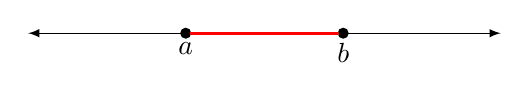
\begin{tikzpicture}
        \draw[latex-latex] (-3,0) -- (3,0); % draws 1-d number line
        \fill[black] (-1,0) circle (2pt) node[below] {$a$}; % draws filled circle at 'a'
        \fill[black] (1,0) circle (2pt) node[below] {$b$}; % draws filled circle at 'b'
        \draw[very thick,red] (-0.95,0) -- (0.95,0); % interval for epsilon neighborhood
    \end{tikzpicture}
\]
Si definisce intervallo aperto di estremi $a$ e $b$ l'insieme $(a,b) =
    \{x\in\mathbb{R}:a<x<b\}$.
\[
    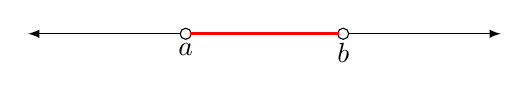
\begin{tikzpicture}
        \draw[latex-latex] (-3,0) -- (3,0); % disegna la retta numerica 1-d
        \draw[black, fill=white] (-1,0) circle (2pt) node[below] {$a$}; % disegna un cerchio vuoto in 'a'
        \draw[black, fill=white] (1,0) circle (2pt) node[below] {$b$}; % disegna un cerchio vuoto in 'b'
        \draw[very thick,red] (-0.95,0) -- (0.95,0); % intervallo per il vicinato di epsilon
    \end{tikzpicture}
\]
%intervalli semiaperti%
Si definisce intervallo chiuso a sinistra e aperto a destra di estremi $a$ e
$b$ l'insieme $[a,b) = \{x\in\mathbb{R}:a\leq x<b\}$.
                \[
                    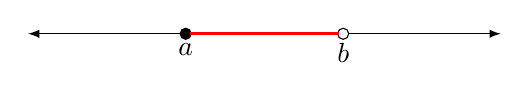
\begin{tikzpicture}
                        \draw[latex-latex] (-3,0) -- (3,0); % disegna la retta numerica 1-d
                        \draw[black, fill=black] (-1,0) circle (2pt) node[below] {$a$}; % disegna un cerchio pieno in 'a'
                        \draw[black, fill=white] (1,0) circle (2pt) node[below] {$b$}; % disegna un cerchio vuoto in 'b'
                        \draw[very thick,red] (-0.95,0) -- (0.95,0); % intervallo per il vicinato di epsilon
                    \end{tikzpicture}
                \]
                Si definisce intervallo aperto a sinistra e chiuso a destra di estremi $a$ e
            $b$ l'insieme $(a,b] = \{x\in\mathbb{R}:a<x\leq b\}$.
\[
    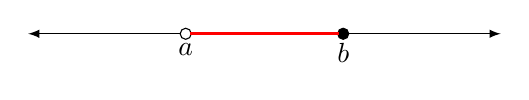
\begin{tikzpicture}
        \draw[latex-latex] (-3,0) -- (3,0); % disegna la retta numerica 1-d
        \draw[black, fill=white] (-1,0) circle (2pt) node[below] {$a$}; % disegna un cerchio vuoto in 'a'
        \draw[black, fill=black] (1,0) circle (2pt) node[below] {$b$}; % disegna un cerchio pieno in 'b'
        \draw[very thick,red] (-0.95,0) -- (0.95,0); % intervallo per il vicinato di epsilon
    \end{tikzpicture}
\]
%intervalli illimitati%
Si definisce intervallo chiuso a sinistra e illimitato superiormente a destra
di estremo $a$ l'insieme $[a,+\infty) = \{x\in\mathbb{R}:a\leq x\}$.
                \[
                    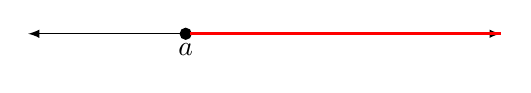
\begin{tikzpicture}
                        \draw[latex-latex] (-3,0) -- (3,0); % disegna la retta numerica 1-d
                        \draw[black, fill=black] (-1,0) circle (2pt) node[below] {$a$}; % disegna un cerchio pieno in 'a'
                        \draw[very thick,red] (-0.95,0) -- (3,0); % intervallo per il vicinato di epsilon
                    \end{tikzpicture}
                \]
                Si definisce intervallo illimitato inferiormente a sinistra e chiuso a destra
                di estremo $a$ l'insieme $(-\infty,a] = \{x\in\mathbb{R}:x\leq a\}$.
\[
    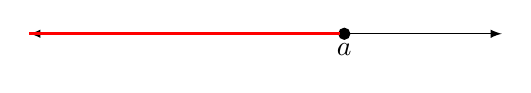
\begin{tikzpicture}
        \draw[latex-latex] (-3,0) -- (3,0); % disegna la retta numerica 1-d
        \draw[black, fill=black] (1,0) circle (2pt) node[below] {$a$}; % disegna un cerchio pieno in 'a'
        \draw[very thick,red] (-3,0) -- (0.95,0); % intervallo per il vicinato di epsilon
    \end{tikzpicture}
\]
Si definisce intervallo aperto a sinistra e illimitato superiormente a destra
di estremo $a$ l'insieme $(a,+\infty) = \{x\in\mathbb{R}:a<x\}$.
\[
    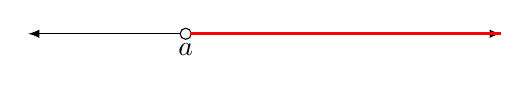
\begin{tikzpicture}
        \draw[latex-latex] (-3,0) -- (3,0); % disegna la retta numerica 1-d
        \draw[black, fill=white] (-1,0) circle (2pt) node[below] {$a$}; % disegna un cerchio vuoto in 'a'
        \draw[very thick,red] (-0.95,0) -- (3,0); % intervallo per il vicinato di epsilon
    \end{tikzpicture}
\]
Si definisce intervallo illimitato inferiormente a sinistra e aperto a destra
di estremo $a$ l'insieme $(-\infty,a) = \{x\in\mathbb{R}:x<a\}$.
\[
    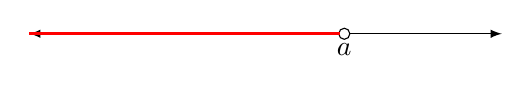
\begin{tikzpicture}
        \draw[latex-latex] (-3,0) -- (3,0); % disegna la retta numerica 1-d
        \draw[black, fill=white] (1,0) circle (2pt) node[below] {$a$}; % disegna un cerchio vuoto in 'a'
        \draw[very thick,red] (-3,0) -- (0.95,0); % intervallo per il vicinato di epsilon
    \end{tikzpicture}
\]
Si definisce intervallo illimitato inferiormente e superiormente
$(-\infty,+\infty) = \mathbb{R}$.
\[
    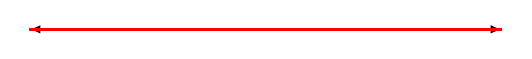
\begin{tikzpicture}
        \draw[latex-latex] (-3,0) -- (3,0); % disegna la retta numerica 1-d
        \draw[very thick,red] (-3,0) -- (3,0); % intervallo per il vicinato di epsilon
    \end{tikzpicture}
\]
\setcounter{part}{2}
\part{Continuità e Discontinuità}
\section*{Continuità}
Sia $f$ una funzione definita in un intervallo aperto $(a,b)$.
Si dice che $f$ è continua in $x_0\in(a,b)$ se
\[
    \lim_{x\to x_0}f(x) = f(x_0)
\]
Si dice che $f$ è continua in $x_0\in(a,b)$ a destra se
\[
    \lim_{x\to x_0^+}f(x) = f(x_0)
\]
Si dice che $f$ è continua in $x_0\in(a,b)$ a sinistra se
\[
    \lim_{x\to x_0^-}f(x) = f(x_0)
\]
Si dice che $f$ è continua in $x_0\in(a,b)$ se è continua sia a destra che a
sinistra.

%Funzioni continue elementari%
\begin{esbox}
    Le funzioni elementari sono continue in ogni punto del loro dominio.
\end{esbox}
\[
    x^a\quad (a\in\mathbb{R});\quad \log x;\quad a^x (a\in\mathbb{R});\quad \sin x;\quad \cos x;\quad |x|
\]
\begin{esbox}
    La funzione $f(x)=x$ è continua in ogni punto del suo dominio.\\ \textit{Funzione identica}
\end{esbox}
Sia $f$ una funzione definita in un intervallo chiuso $[a,b]$.
Si dice che $f$ è continua in $a$ se
\[
    \lim_{x\to a^+}f(x) = f(a)
\]
Si dice che $f$ è continua in $b$ se
\[
    \lim_{x\to b^-}f(x) = f(b)
\]
%Continuità di funzioni somma, prodotto, quoziente, composizione%
Prese due funzioni $f$ e $g$ continue in $x_0$, allora
\begin{itemize}
    \item $f+g$ è continua in $x_0$;
    \item $f-g$ è continua in $x_0$;
    \item $f\cdot g$ è continua in $x_0$;
    \item $f/g$ è continua in $x_0$ se $g(x_0)\neq 0$;
    \item $f(g(x))$ è continua in $x_0$ se $g$ è continua in $x_0$ e $f$ è continua in $g(x_0)$.
\end{itemize}
Osserva che in un punto isolato la funzione è continua.\\
%Criterio di monotonia%
\section*{Criterio di monotonia}
Sia $f$ una funzione continua in un intervallo $[a,b]$ e derivabile in $(a,b)$. Allora.
\begin{itemize}
    \item Se $f'(x)\geq 0$ in $(a,b)$, allora $f$ è crescente in $[a,b]$.
    \item Se $f'(x)\leq 0$ in $(a,b)$, allora $f$ è decrescente in $[a,b]$.
    \item Se $f'(x)> 0$ in $(a,b)$, allora $f$ è strettamente crescente in $[a,b]$.
    \item Se $f'(x)< 0$ in $(a,b)$, allora $f$ è strettamente decrescente in $[a,b]$.
    \item Se $f'(x)= 0$ in $(a,b)$, allora $f$ è costante in $[a,b]$.
\end{itemize}
\newpage
\section*{Discontinuità}
Sia $f$ una funzione definita in un intervallo aperto $(a,b)$. Si dice che $f$
è discontinua in $x_0\in(a,b)$ se non è continua in $x_0$. In particolare, si
dice che $f$ è discontinua in $x_0\in(a,b)$ se
\[
    \lim_{x\to x_0^+}f(x) \neq \lim_{x\to x_0^-}f(x) \quad \textbf{\textit{Discontinuità di prima specie o di salto}}
\]
$x_0$ è un punto di discontinuità di prima specie se i limiti destro e sinistro della funzione in $x_0$ esistono e sono finiti ma sono diversi.
\begin{figure}[h]
    \centering
    \includegraphics[width=0.5\textwidth]{discsalto.png}
    \caption{Discontinuità di prima specie o di salto}
\end{figure}
\[
    \lim_{x\to x_0^+}f(x) = \pm\infty \quad \lor \quad \lim_{x\to x_0^-}f(x) = \pm\infty \quad \text{oppure}\]
\[
    \quad \lim_{x\to x_0^+}f(x) = \nexists \quad \lor \quad \lim_{x\to x_0^-}f(x) = \nexists \quad \textbf{\textit{Discontinuità di seconda specie}}
\]
$x_0$ è un punto di discontinuità di seconda specie se almeno uno tra limite sinistro o destro della funzione in $x_0$ è uguale a $\pm\infty$, oppure non esiste.
\begin{figure}[h]
    \centering
    \includegraphics[width=0.5\textwidth]{discsecond.png}
    \caption{Discontinuità di seconda specie}
\end{figure}
\\Ricordiamo che una funzione monotona può avere al più un numero finito di punti di discontinuità di prima specie.\\
\newpage
\[
    \lim_{x\to x_0}f(x) \neq f(x_0) \quad \textbf{\textit{Discontinuità di terza specie o eliminabile}}
\]
$x_0$ è un punto di discontinuità di terza specie se il limite sinistro e destro della funzione in $x_0$ sono uguali e
finiti ma non esiste il valore della funzione in $x_0$ oppure esiste ma risulta diverso dal limite cioè diverso dal suo limite destro e sinistro.\\
\begin{figure}[h]
    \centering
    \includegraphics[width=0.5\textwidth]{discelim.png}
    \caption{Discontinuità di terza specie o eliminabile}
\end{figure}
\\In questo caso la discontinuità si può eliminare ponendo $f(x_0)=\lim_{x\to x_0^+}f(x)=\lim_{x \to x_0^-}f(x)$.
\end{document}
